\documentclass[bachelor, subf,href,colorlinks=true
%,times        % шрифт Times как основной
%,fixint=false % отключить прямые знаки интегралов
]{disser}

\usepackage[
  a4paper, mag=1000, includefoot,
  left=3cm, right=1cm, top=2cm, bottom=2cm, headsep=1cm, footskip=1cm
]{geometry}
\usepackage{color}
\usepackage[TS1, T2A]{fontenc}
\usepackage[utf8]{inputenc}
\usepackage[english,russian]{babel}
\ifpdf\usepackage{epstopdf}\fi
\usepackage{graphicx}
% Номера страниц сверху и по центру
%\def\headfont{\small}
%\pagestyle{headcenter}
%\chapterpagestyle{empty}

% Точка с запятой в качестве разделителя между номерами цитирований
%\setcitestyle{semicolon}
% Использовать полужирное начертание для векторов
\let\vec=\mathbf

% Включать подсекции в оглавление
\setcounter{tocdepth}{2}

\graphicspath{{fig/}}
\usepackage{cmap}
\usepackage{listings}
\lstloadlanguages{C++, bash, Python, Java, PHP, Pascal}
 \lstset{inputencoding=utf8, breaklines=true, extendedchars=false, numbers=left, language=C++,
       frame=rl, rulesepcolor=\color{black}
       }
\renewcommand{\lstlistingname}{Листинг}

\begin{document}

\institution{Санкт-Петербургский государственный
электротехнический университет «ЛЭТИ» им. В.И. Ульянова (Ленина) (СПбГЭТУ)}


% Имя лица, допускающего к защите (зав. кафедрой)
\apname{Советов Борис Яковлевич}

\title{ВЫПУСКНАЯ РАБОТА\\БАКАЛАВРА}


\topic{Использование динамических библиотек в рамках Flash-приложений}


% Автор
\author{Борисенко Константин Алексеевич} % ФИО
\group{8372} % Группа
\coursenum{,,,,,} % Номер специальности
\course{..........} % Название специальности


% Научный руководитель
\sa      {Степуленок Денис Олегович}
\sastatus{асс. каф. АСОиУ СПБГЭТУ}



% Город и год
\city{Санкт-Петербург}
\date{\number\year}

\maketitle
\begin{center}
\textbf{Аннотация}
\end{center}
В данной дипломной работе разработан программный продукт, представляющий собой web-сервер на базе Node.js, который позволяет вызывать функции, реализованнные в динамической библиотеке из Flash-приложений или других технологий (например, Javascript, Silverlight) для создания клиентской части web-приложения.\\
В дипломной работе разработана общая схема системы, проанализированы достоинства и недостатки возможных средств реализации, и выбрано наилучшее с точки зрения сформулированных критериев. \\
С целью сравнения приведены листинги web-серверов, реализованных на разных языках (C, Python, PHP, Node.js).\\
Разработан исходный код сервера на Node.js, описан процесс настройки Node.js под Linux.\\
Эту работу можно использовать для дальнейшей разработки задач КИО на Flash, требующих использование функций из динамических библиотек. \\
В заключении описаны возможные перспективы программного продукта. Большая часть поставленных в техническом задании целей была достигнута.

\newpage
\begin{center}
\textbf{Abstract}
\end{center}
In this diploma has been created a software, which is a server made on Node.js, which allows to connect dynamic libraries with Flash-applications or other techono-logies (ex. Javascript, SilverLight) for making client parts of web-services.\\
The common structure of the client has been shown, advantages and disadvantages of possible platforms has been analyzed, and the best solution according to formula-ted criteria has been chosen.\\
In order to compare listings of web-servers, made on C, Python, PHP, Node.js has been demonstrated.\\
The project has been made on Node.js. Process of setting-up Node.js on Linux has been shown.\\
This project can be useful for the future development of the competition CEO (to Construct, to Explore, To optimize) on Flash.\\
In the end there are future possibilities of this product. Allmost all of the goals, described in specification, has been reached.

\newpage
\begin{center}
\textbf{Ключевые слова}
\end{center}
\begin{itemize}
  \item Node.JS
  \item Javascript
  \item Создание, вызов динамической библиотеки
  \item Flash
  \item ActionScript
  \item Flash player debugger
  \item npm
  \item node-ffi
\end{itemize}
\tableofcontents
\chapter{Системный анализ предметной области и постановка задачи }
\section{Предметная область}
Существует конкурс КИО - «Конструируй, Исследуй, Оптимизируй» (рис. ~\ref{KIOemblem}). Он был создан 9 лет назад. Данный конкурс проводится для учеников с 1 по 11 класс. Существует три уровня: 
 \begin{itemize}
        \item начальный уровень - для учеников начальных классов,
        \item уровень I - для учеников от 5 до 7 класса включительно,
        \item уровень II - для старших участников. 
    \end{itemize}


\begin{figure}[h]
\begin{minipage}[h]{0.49\linewidth}
\center{
\includegraphics[width=0.5\linewidth]{KIOemblem1} \\ а)}
\end{minipage}
\hfill
\begin{minipage}[h]{0.49\linewidth}
\center{
\includegraphics[width=0.5\linewidth]{KIOemblem2} \\ б)}
\end{minipage}
\caption{Эмблемы конкурса КИО}
\label{KIOemblem}
\end{figure}

Участникам каждого уровня предлагаются три логические задачи. Все задачи отражают недавно возникшее направление научных исследований, которое, применительно к разным наукам, получило названия компьютерной математики, компьютерной физики, компьютерной биологии и т. д. За каждым игровым сюжетов стоит серьёзная и, возможно, ещё не решённая в общем виде задача, которая после окончания Конкурса подробно и популярно обсуждается на страницах журнала «Компьютерные инструменты в школе».
Задания конкурса представлены в форме компьютерных моделей-лабораторий с игровыми элементами. В процессе работы с заданием участник конструирует частичные решения задачи, которые оцениваются по установленным в задании критериям. Таким способом формируется «рекорд» - число или набор чисел, характеризующие степень достижения поставленных в задании целей. Механизм рекорда позволяет участникам оценивать собственное продвижение в решении задач, а для жюри конкурса рекорды являются основой для составления рейтинга. 
Конкурс позволяет ребятам из самых отдаленных уголков России участвовать наравне с ребятами из больших городов, если у них есть Интернет или электронная почта. 
По окончании Конкурса каждый участник получает электронный сертификат, заверенный электронной подписью. Это означает, что выдаваемый жюри Конкурса электронный сертификат зашифрован так, что его можно проверить на подлинность открытием в программе «Электронный сертификат» на сайте Конкурса, но подделать его невозможно.
Я учавствовал в создании Конкурса КИО-2010. Я создал логическую задачу "Прожорливый тьюрмит". Для меня это был бесценный опыт, и я с радостью учавствую в модернизации Конкурса сейчас. Созданная мною игра будет описана в примерах задач.
Далее приведены примеры задач.
\subparagraph{Прожорливый тьюрмит (рис. ~\ref{ant})}
Существо, которое в теории алгоритмов называют тьюрмитом (Тьюринг+термит), перемещается по тору, развертка которого представлена в виде клетчатого поля 20x20. Тор, который мы может представить в виде бублика, получится из этого поля, если его «свернуть в трубочку», а затем соединить края трубки. При этом соседними станут верхние и нижние клетки каждого столбца и каждой строки исходного поля.

Управляется тьюрмит автоматом, графическое  изображение которого находится справа. Каждый кружок представляет собой состояние, в котором находится в данный момент «мозг» тьюрмита, а стрелочки между состояниями соответствуют действиям тьюрмита в той или иной ситуации.

Всего ситуаций, по которым «мозг» тьюрмита принимает решения, две – есть ли яблоко перед ним или нет. В каждой из ситуаций тьюрмит может совершить три действия: пойти прямо и перейти в следующую клетку, повернуться вправо или влево. Если в клетке, в которую попадает тьюрмит, находится яблоко, то он съедает его.

Ваша  задача состоит в том, чтобы сконструировать  такой «мозг» тьюрмита, который позволит ему за 130 шагов съесть как можно больше яблок. При одинаковом числе съеденных яблок лучшей считается та конструкция автомата, которая имеет меньшее число состояний. Обратите внимание на то, что тьюрмит может сделать много шагов, находясь в одном состоянии. В этом случае автомат будет иметь петлю, начинающуюся и заканчивающуюся в этом состоянии.
\begin{figure}[!ht]
	\begin{center}
		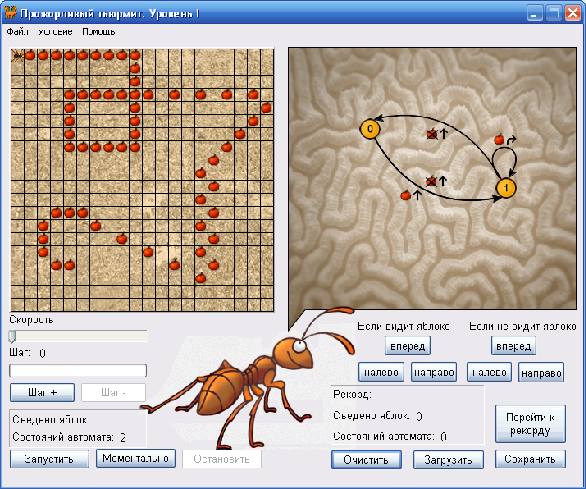
\includegraphics[]{ant}
	\end{center}
	\caption{Прожорливый тьюрмит}
	\label{ant}
\end{figure}


\subparagraph{Освещение города.}
Демонстрация полностью настраиваемых окружений типа <<теорема>>.
Муниципалитет маленького городка хочет сэкономить на освещении улиц. Помогите ему разработать схему освещения, расставив фонари так, чтобы они осветили все закоулки города, но число фонарей при этом было минимальным (рис. ~\ref{town_light1}).
\begin{figure}[!ht]
	\begin{center}
		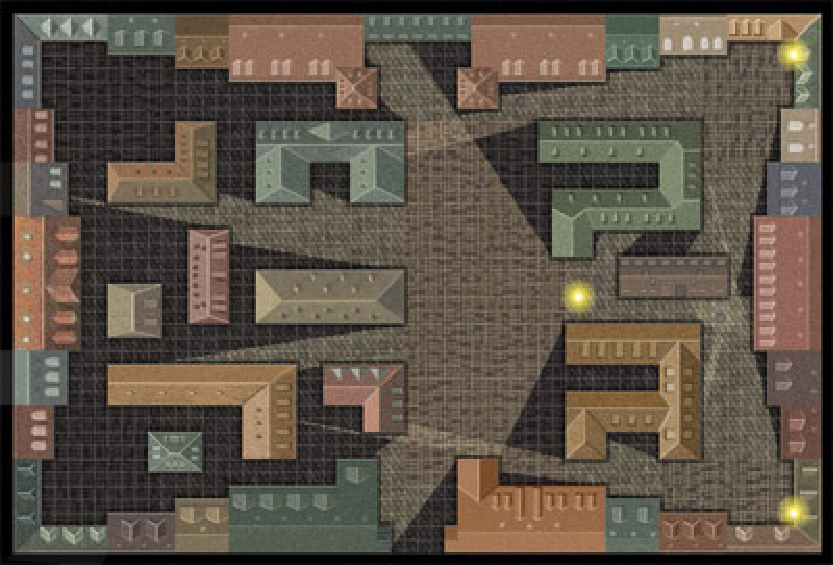
\includegraphics[]{town_light1}
	\end{center}
	\caption{Освещение города}
	\label{town_light1}
\end{figure}

\subparagraph{Сезам, откройся!}
От каждого путника, желающего добыть новое сокровище горы Сезам, Дух Горы требует принести несколько серебряных монет. По своему усмотрению Дух обращает часть монет в золотые монеты желтого золота, а остальные - в монеты красного золота, которые немного тяжелее монет из желтого золота. При этом Дух никогда не превращает все монеты в золотые одного вида. Путника, принесшего монеты, Дух испытывает задачей. Он просит не более четырёх раз положить равное число монет на разные чашки весов так, чтобы после превращения монет в золотые равновесие весов хотя бы раз нарушилось. При этом хитрый Дух всегда старается так превращать монеты в два вида золотых, чтобы при всех взвешиваниях весы оставались в равновесии. Вы должны перехитрить Духа и указать такой алгоритм взвешиваний, при котором для выбранного вами числа монет равновесие всегда нарушается (рис. ~\ref{open_sesame}).
\begin{figure}[!ht]
	\begin{center}
		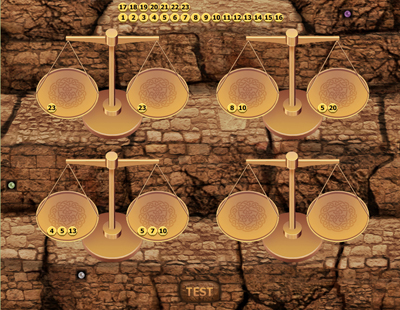
\includegraphics[]{open_sesame}
	\end{center}
	\caption{Сезам, откройся}
	\label{open_sesame}
\end{figure}
\subparagraph{Математическое скалолазание.}
Известно, что многие известные ученые занимались альпинизмом. Однажды они устроили соревнование по скалолазанию по необычным правилам. Одна команда забивает в скалу 16 крючьев, а другая соединяет крючья веревкой без пересечений так, чтобы потом как можно скорее пройти по ней весь маршрут. Считается, что по всем участкам маршрута скалолазы движутся с одной скоростью, поэтому вторая команда всегда прокладывает веревку по крючьям так, чтобы минимизировать длину маршрута. Наоборот, команда, забивающая крючья, должна позаботиться о том, чтобы даже самый короткий маршрут, проложенный по ним, был как можно длиннее. Ваша задача – вбить крючья так, чтобы максимально усложнить задачу сопернику(рис. ~\ref{rock_climber1}).
\begin{figure}[!ht]
	\begin{center}
		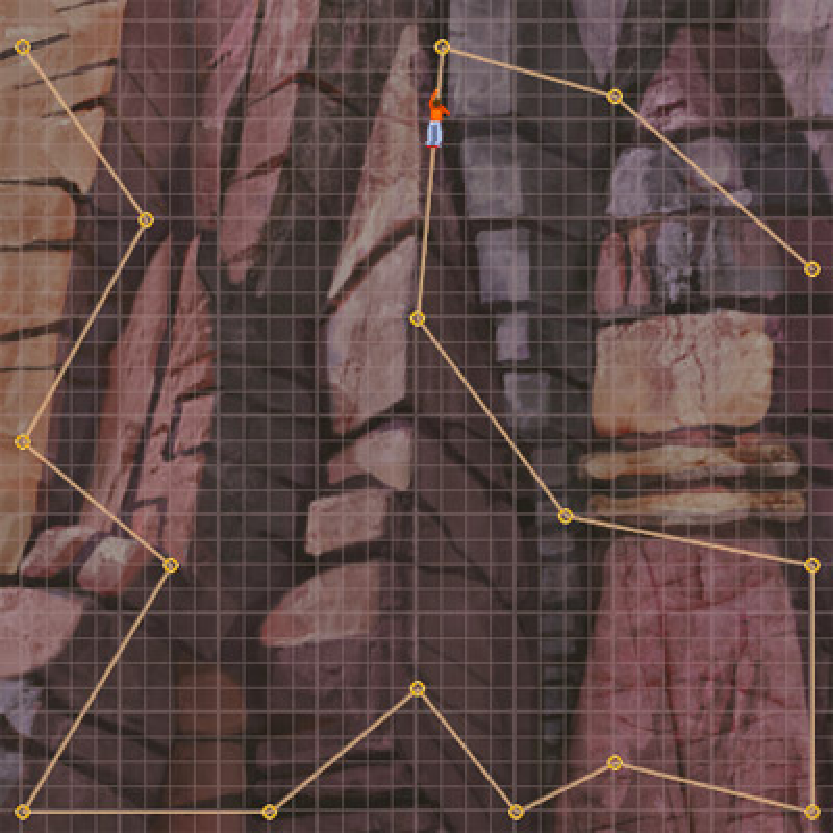
\includegraphics[]{rock_climber1}
	\end{center}
	\caption{Математическое скалолазание}
	\label{rock_climber1}
\end{figure}

До 2011 года все задачи создавались на языке Delphi. Начиная с 2011 года задачи стали делать на Flash. Flash — удобная кроссплатформенная среда для создания проектов. Так как во многих школах России теперь устанавливается СПО — свободное программное обеспечение, и, соответственно, ставится Unix подобные системы, то конкурс в виде exe-файла перестал быть легкодоступен для всех желающих участников. Для Flash-приложений же достаточно лишь наличие браузера и Flash Player'а. В этом году появилась возможность использовать динамическую библиотеку, созданную в ИТМО, которая позволяет облегчить серьёзные математические вычисления, которые приходится производить при создании подобных проектов. Возникла проблема в том, что Flash не может напрямую использовать динамические библиотеки. 


\section{Постановка задачи дипломного проекта}
При создании различных приложений часто требуются математические и другие пакеты, которые уже реализованы в виде динамических библиотек, и создавать их заново, используя, например, Flash, слишком затратно. То есть существует потребность использовать из Flash-приложений уже имеющиеся динамические библиотеки. Решение данной проблемы касается не только Flash-приложений, а любых других платформ, используемых для создания клиентской части веб-приложения (Javascript, SilverLight, PHP, Python, Ruby).
Напрямую из Flash нет возможности обращаться к динамическим библиотекам. Цель диплома - разработать компоненты, которые позволили бы использовать динамический библиотеки из Flash.
Если был бы доступен исходных код библиотек, то можно было бы его адаптировать к вызову из Flash. В данном случае это будет неуниверсальный способ и при любых изменениях в динамической библиотеке, адаптацию придётся проводить заново. Нужно найти универсальный способ, который будет работать при подключении любой динамической библиотеки.
Требованию к разрабатываему продукту:
\begin{itemize}
  \item Время на вызов функции через созданные в дипломе модули не должно отразиться на общей скорости приложения. Замедление работы программы не должно быть заметно пользователю;
  \item Весь проект должен занимать как можно меньше места, так как его будут скачивать участники со всех уголков России, у которых пропускная способность интернет-канала может быть слишком слабой для больших файлов. То есть увеличение размера не должно превышать нескольких мегабайт.
  \item Проект должен работать как под Windows, так и в различных дистрибутивах Linux;
  \item Из динамической бибилиотеки требуется вызывать функции. Каждая функция задаётся ее именем, типом возвращаемого значения, и типами аргументов.
  \item Исходный код должен быть понятен и прокомментирован.
\end{itemize}
\chapter{Используемые технологии}
\section{Структура проекта}
Так как исходных кодов библиотек нет, значит возможности перевести их на ActionScript нет. Было принято решение использовать виртуальный сервер для связи Flash с динамическими библиотеками. На рис. ~\ref{scheme1} представлена схема работы нашего проекта.\\
\begin{figure}[!ht]
	\begin{center}
		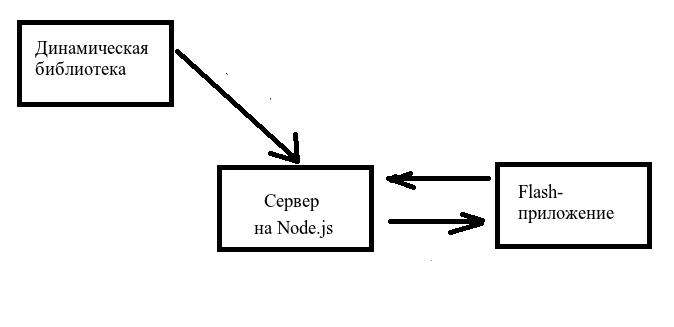
\includegraphics[width=12cm]{schemeOfCommunic}
	\end{center}
	\caption{Схема связи Динамической библиотеки и Flash-приложения}
	\label{scheme1}
\end{figure}

Этапы запуска приложения:
 \begin{itemize}
        \item Запуск сервера,
        \item Иницилизация динамической библиотеки,
        \item Запуск Flash-приложения;
    \end{itemize}

После этого Flash-приложение посылает запрос серверу на выполнение той или иной, загруженной из динамической библиотеки, функции. Сервер обрабатывает запрос, выполняет нужную функцию с полученными из запроса параметрами, и посылает ответ клиенту (Flash-приложению). 
Данная схема позволяет Flash-приложениям использовать динамические библиотеки.

\section{Выбор платформы для Flash}
В качестве среды программирования мною был использована среда IntelliJ IDEA (рис. ~\ref{inteliJ}).
\begin{figure}[!ht]
	\begin{center}
		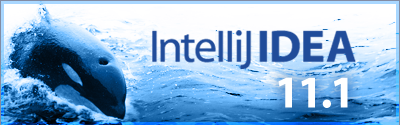
\includegraphics[width = 8cm]{intelliJ}
	\end{center}
	\caption{Эмблема IntelliJ IDEA}
	\label{inteliJ}
\end{figure}
Она была выбрана, так как является удобной платформой для создания приложений, в ней существует большой набор мощных инструментов, не навязывающих определенных структур проекта, имеет удобный редактор. В качестве компилятора был выбран Flex SDK. По сравнению с компилятором Adobe Flash, он имеет удобный debugger, сохраняя при этом все возможности Flash. В отличие от Adobe Flash Flex SDK распространяется бесплатно.

\section{Выбор платформы для создания сервера}
\subsection{Протокол передачи} 
В качестве протокола передачи информации был выбран http-протокол, потому что он, как правило, не должен перекрываться для передачи информации. Это происходит, потому что для открытия веб-страницы в интернете требуется этот протокол, следовательно ни в какой операционной системе он не запрещён к использованию.
Также в ActionScript существует класс URLLoader, который относится к пакету flash.net. Данный класс может создавать http-запросы и принимать их в виде текста, двоичных данных или переменных в кодировке URL. Методы данного класса полностью удовлетворяет потребностям проекта.

\subsection{Среда создания}
Сервер может располагаться локально на компьютере участника, либо находиться удаленно.
Было принято решение размещать сервер локально на каждом компьютере, на котором будет устанавливаться пакет конкурса КИО. Плюсы данного варианта заключаются в том, что участникам не нужно постоянное устойчивое соединение с удалённым сервером для посылки запросов. Тем самым, ученики могут скачать установщик и учавствовать в конкурсе, пользуясь компьютерами без выхода в интернет. Минус — нужно найти такой сервер, который не будет занимать много места, будет быстро скачиваться, и будет легок в настройке, быстр в использовании.
Существует большое количество платформ и языков программирования для создания серверов, а именно: 
C++, PHP, node.js, python. 
Рассмотрим примеры создания серверов на этих платформах. 
\paragraph{Сервер на С++}
В листинге ~\ref{httpC} реализован простой http-сервер, который на успешный запрос клиента отвечает, что сообщение было получено. Программисту, который никогда не сталкивался с созданием серверов будет достаточно сложно разобраться в назначении многих параметров и вообще структуры создания сервера на C++.

В тоже время сервер на C++ является хорошим вариантом для нашего проекта, так как он не будет занимать много места на жёстком диске и будет достаточно быстр при обработке для наших условий.
 \lstinputlisting[frame=shadowbox,
   emph={forsuffixes,text,bpath},emphstyle={\color{red}},
   emph={[2]fill,unfill},emphstyle={[2]\bfseries\underbar}, caption=Пример http-сервера на С++, label={httpC}
 ]{httpC.c}

\paragraph{Сервер на PHP}
Теперь рассмотрим пример http-сервера на PHP. Последняя версия PHP 5.4 содержит встроенный веб-сервер, соответственно не требуется установка Apache или других аналогичных серверов, которые сложны в настройке.
Запускается сервер следующим образом. Пример для Linux:
 \begin{lstlisting}[numbers=none, language=bash]
	$ php -S localhost:8000
\end{lstlisting}
В консоли выведется следующее:
 \begin{lstlisting}[numbers=none, language=bash]
	PHP 5.4.0 Development Server started at Date
	Listening on localhost:8000
	Document root is /home/username/
	Press Ctrl-C to quit
\end{lstlisting}
Скрипт index.php будет выглядеть так:
 \begin{lstlisting}[numbers=none, language=PHP]
<?
  echo "Hello world!";
\end{lstlisting}
На каждый запрос, посланный серверу, будет выдаваться содержимое index.php, в данном примере будет выводиться Hello world!

\paragraph{Сервер на Python}
В коде листинга ~\ref{httpPython} сервер обрабатывает запрос, и при успешном запросе выдаёт клиенту запрошенную страницу.
 \lstinputlisting[frame=shadowbox, language=Python,
   emph={forsuffixes,text,bpath},emphstyle={\color{red}},
   emph={[2]fill,unfill},emphstyle={[2]\bfseries\underbar}, caption=Пример http-сервера на Python, label={httpPython}
 ]{httpPython.py}

Сервер на Python умеет отвечать на запрос с именем страницы выводом самой страницы.

\paragraph{Сервер на Node.js}
Node.js — это сравнительно новая платформа, построенная на основе  Chrome's JavaScript Runtime для легкого создания быстрых, масштабируемых сетевых приложений. Node.js позволяет выполнять Javascript-код вне браузера. Он состоит из среды исполнения программ и большого количество дополнительных библиотек. Листинг ~\ref{httpNodejs} отражает код для создания сервера на Node.js
 \lstinputlisting[frame=shadowbox, language=Java,
   emph={forsuffixes,text,bpath},emphstyle={\color{red}},
   emph={[2]fill,unfill},emphstyle={[2]\bfseries\underbar}, caption=Пример http-сервера на Node.js, label={httpNodejs}
 ]{httpNode.js}

Все. Вот и весь сервер. На каждый запрос он выводит Hello World. Очень просто и понятно. К неоспоримым плюсам относится то, что процесс node.js живёт долго и обрабатывает все http-запросы внутри себя. Это значит, что для каждого нового запроса не выполняется инициализация, как, например, на PHP. А это существенно сокращает время обработки запросов. С помощью таких инструментов как The Node Toolbox (http://toolbox.no.de/) и npm (http://npmjs.org/) процесс поиска, выбора и установки необходимых модулей становится простым и быстрым. Также очень понравилась документация, которая существует не только на английском, но и на русском языках.

Заглядывая в будущее, если предположить, что сервер будет запускаться удалённо, тогда не нужна никакая настройка сервера локально на каждом компьютере. Но тогда будет возникать проблема перегруженности сервера, ведь в предыдущие года в конкурсах участвовали более 60 тысяч учеников и их число каждый год растёт. \\

Node.js выполняет все запросы асинхронно. Если какой-то запрос приходит на сервер, а сервер уже занят обработкой другого процесса, то новый запрос всё равно сразу же начнёт выполняться. Быстродействие node.js впечатляет.\\
Приведу сравнительный анализ, представленный на сайте \\
http://b.brainscode.com/2011/04/nodejs-vs-php.html. В этом анализе сравнивается быстродействия node.js и php. Проведем тесты на простых математических вычислениях. В листингах ~\ref{phpTest} и ~\ref{nodejsTest} предсталены скрипты тестов на PHP и Node.js соответственно.
 \lstinputlisting[frame=shadowbox, language=PHP,
   emph={forsuffixes,text,bpath},emphstyle={\color{red}},
   emph={[2]fill,unfill},emphstyle={[2]\bfseries\underbar}, caption=Тестовый скрип php, label={phpTest}
 ]{phpTest.py}
 \lstinputlisting[frame=shadowbox, language=Java,
   emph={forsuffixes,text,bpath},emphstyle={\color{red}},
   emph={[2]fill,unfill},emphstyle={[2]\bfseries\underbar}, caption=Тестовый скрип Node.js, label={nodejsTest}
 ]{nodejsTest.js}

Таблица ~\ref{testTable} показывает результаты тестов.

\begin{center}
\begin{tabular}{|c|c|c|}
\hline
  & \multicolumn{2}{|c|}{\textbf{Время (сек.)}}\\
\hline
\textbf{Кол-во итераций} &   \textbf{Php}     &  \textbf{Node.js}\\
\hline
100 000 & 0.077 & 0.02\\
\hline
1 000 000 & 0.759 & 0.016\\
\hline
10 000 000 & 7.605 & 0.157\\
\hline
100 000 000 & 75.159 & 1.567\\
\hline
\end{tabular}
\end{center}
\tablecaption{Таблица ~\ref{testTable}. Сравнение быстродействия PHP и Node.js} \label{testTable}

Как видим nodejs существенно превосходит в данном тесте, при самой большой размерности выигрыш в времени выходит почти в 50 раз, при значении в 100 000 раз этот показатель равен — 38 соответственно. Выигрыш, как видно существенный.
Также в видео-лекции Ryan'а Dahl'а (одного из создателей Node.js) показано, что если создан сервер, который на каждый запрос отвечает двух-секундной задержкой (см. ~\ref{dahl}), то при 100 000 одновременных запросах время обработки запросов сервером будет составлять чуть более 2 секунд, что свидетельствует о параллельной обработке запросов, об асинхронной работе сервера.\begin{lstlisting}[numbers=none, language=bash, caption =Тело функции обработки запроса в Node.js,
 			label=dahl]
  setTimeout(function(){
	console.log("hello world");
}, 2000);
\end{lstlisting}

И, в конце-концов, программы на Javascript являются легко читаемыми.

По вышеперечисленным причинам было принято решение использовать сервер, созданный на node.js. Из минусов можно отметить, что сервер будет занимать чуть менее 5 мб, но, учитывая все достоинства использования Nodejs, этим минусом можно пренебречь. Даже если предположить, что у участника интернет типа dial-up с максимальной скоростью 64 кбит/сек:
\begin{itemize}
 \item 64 кбит/сек = 8 кбайт/сек;
  \item 5 мбайт = 5120 кбайт  (максимальный размер сервера)
  \item 5120 / 8 = 640 сек;
  \item 640 / 60 = 10 минут 40 секунд - худший расклад.
\end{itemize}
При скорости 512 кбит/сек (64 кбайт/сек) время закачки будет равно 80 секундам.
\subsection{Создание тестовой динамической библиотеки}\label{CreationDynLib}
Также для создания тестовой динамической библиотеки будет использоваться Microsoft Visual Studio 2010 Express для Windows и компилятор gcc на Linux.
В листинге ~\ref{big.c} приведен код, из которого комплируется динамическая библиотека.
 \lstinputlisting[frame=shadowbox, language=Java,
   emph={forsuffixes,text,bpath},emphstyle={\color{red}},
   emph={[2]fill,unfill},emphstyle={[2]\bfseries\underbar}, caption=Код компилируемой динамической библиотеки, label={big.c}
 ]{../f1.c}
Чтобы создать динамическую библиотеку в Linux нужно сначала скомпилировать файл big.c. Для этого в терминале вводим следующее:
\begin{lstlisting}[numbers=none, language=bash]
    gcc -fPIC -с big.c
\end{lstlisting}
Ключ -fPIC включен, потому что мы создаём динамическую библиотеку. Это нужно для того, чтобы переходы в функциях использовали не абсолютную адресацию, а относительную, иначе несколько различных программ не смогут использовать эту библиотеку.
В результате мы получаем файл big.o, который используем следующим образом:
\begin{lstlisting}[numbers=none, language=bash]
    gcc -shared -o big.o
\end{lstlisting}
В результате будет получен файл big.so, который и будет являться динамической библиотекой, используемая далее в проекте.
\newpage
\section{Структура проекта}
После того как все языки программирования были выбраны, структура проекта будет иметь вид как на рис. ~\ref{schemeWithBranch}. К Node.js подключается дополнительная библиотека node-ffi для работы с динамическими библиотеками. Общение Flash-приложения с сервером происходит через http-запросы и http-ответы. 
Библиотека node-ffi является дополнительной библиотекой Node.js, которая работает с динамическими библиотеками. Принцип ее работы описан в разделе ~\ref{ServerPart}.

\begin{figure}[!ht]
	\begin{center}
		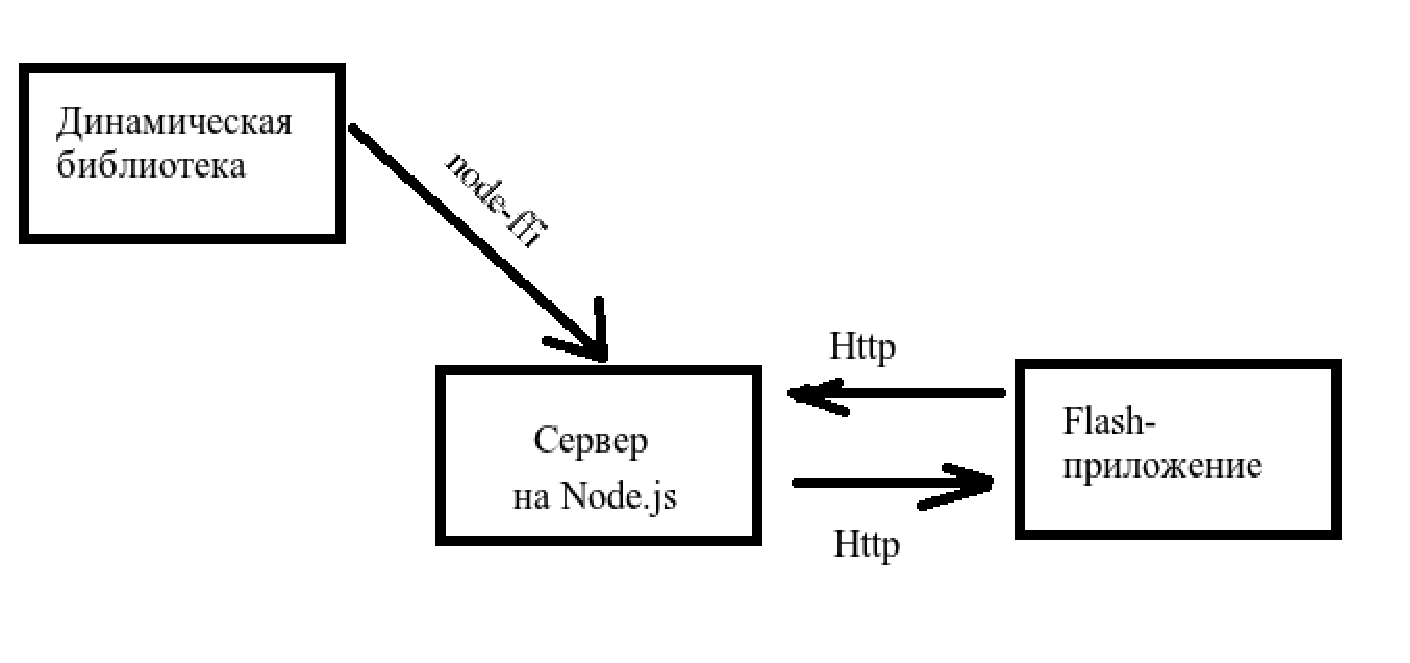
\includegraphics[width=12cm]{schemeOfCommunicWithBranches}
	\end{center}
	\caption{Структура проекта со связями}
	\label{schemeWithBranch}
\end{figure}
\chapter{Проектирование}
\section{Настройка Node.js}
\subsection{Настройка под Linux}\label{OnLinuxInstall}
В данном разделе описывается установка Node.js на Ubuntu 11.10.
Устанавливаем сам nodejs:
\begin{lstlisting}[numbers=none, language=bash]
	$ sudo apt-get install nodejs
\end{lstlisting}
Далее устанавливаем пакетный менеджер npm (Node Package Manager):
\begin{lstlisting}[numbers=none, language=bash]
	$ sudo apt-get install npm
\end{lstlisting}
Перед установкой node-ffi должен быть установлен Python (он уже по умолчанию стоит на Ubuntu 11.10). Если требуется установка, то также используется пакетный менеджер (рекомендуемая версия Python 2.7.2).
Также должен быть установлен C/C++ компилятор, например, gcc:
\begin{lstlisting}[numbers=none, language=bash]
	$ sudo apt-get install gcc
\end{lstlisting}
После предварительных установок устанавливаем node-ffi:
\begin{lstlisting}[numbers=none, language=bash]
	$ npm install ffi
\end{lstlisting}
Если установка не прошла успешна, а все предыдущие шаги были выполнены верно, то значит в операционной система используется библиотека libffi не той версии, которая нам нужна. Такая проблема возникла в Ubuntu 11.10. При установке на Ubuntu 12.04 такой проблемы нет. Соответственно тогда удаляем старую библиотеку:
\begin{lstlisting}[numbers=none, language=bash]
	$ sudo apt-get remove libffi4
\end{lstlisting}
И устанавливаем  (libffi-dev, если libffi нет):
\begin{lstlisting}[numbers=none, language=bash]
	$ sudo apt-get install libffi
\end{lstlisting}
После этого снова повторяем установку node-ffi.
\subsection{Настройка под Windows}\label{windowsInstall}
Для установки Node.js достаточно скачать установщик с официального сайта программы (nodejs.org) и установить его. На данном этапе проекта подключить node-ffi к проекту в Windows не удалось. 
Далее представлены испробованные способы установки.
\paragraph{Установка, используя документацию, приложенную к библиотеке node-ffi.}
Предварительно под Windows нужно установить python 2.7.2, также Microsoft Visual Studio C++, разработчики рекомендуют последнюю версию на данный момент, а именно Visual C++ 2010 Express. Также для 64-х битных систем нужно установить Windows 7 64-bit SDK.
После установки всего в командной строке была произведена попытка установки node-ffi через npm (npm install node-ffi). На рис. ~\ref{sh_error} представлена ошибка, возращаемая при таком способе установки. 
\begin{figure}[!ht]
	\begin{center}
		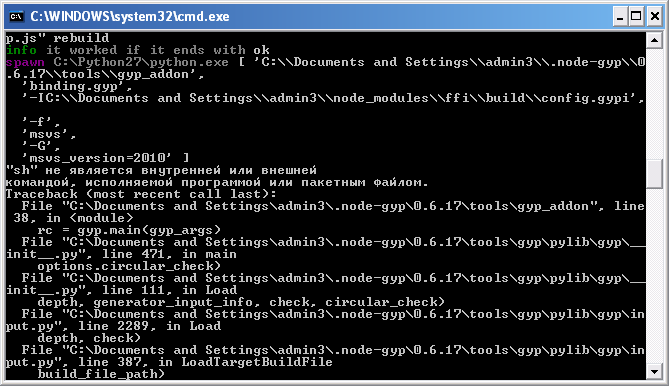
\includegraphics[width=11cm]{SH_error}
	\end{center}
	\caption{Ошибка при установке node-ffi через npm в командной строке}
	\label{sh_error}
\end{figure}
SH — Shell Script — скрипт, в котором представлены наборы команд для последовательного выполнения команд в командной строк Unix-подобных систем. Соответственно, под Windows данная команд на выполнение скрипта не будет выполняться.
\newpage

\paragraph{Установка с помощью "Установщика веб-платформы".}
Данная программа является аналогом пакетного менеджера в Unix-подобных системах. Скачать её можно на сайте:\\
 http://www.microsoft.com/web/downloads/platform.aspx (рис. ~\ref{installer_web})
\begin{figure}[!ht]
	\begin{center}
		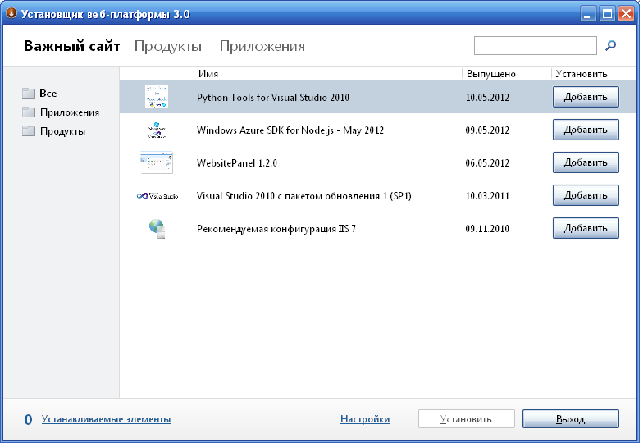
\includegraphics[width=11cm]{installer_web}
	\end{center}
	\caption{Установщик веб-платформы 3.0}
	\label{installer_web}
\end{figure}
Для установки node.js через установщик нужно установить рабочее окружение. 
Устанавливаем рекомендуемую конфигурацию IIS 7. 
Заходим в Настройки и добавляем сайт, на котором можно скачать nodejs: \\ http://www.helicontech.com/zoo/feed (рис. ~\ref{properties_web}).
\begin{figure}[!ht]
	\begin{center}
		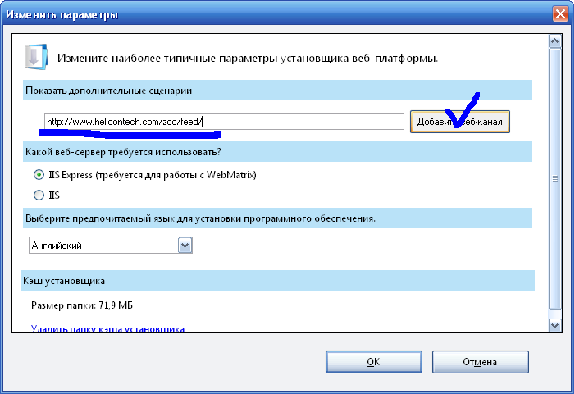
\includegraphics[width=11cm]{properties_web}
	\end{center}
	\caption{Добавление сайта, содержащего пакет установки Node.js}
	\label{properties_web}
\end{figure}
После этого на вкладке Zoo устанавливаем в разделе Packages, как показано на рис. ~\ref{package_web}.
\begin{figure}[!ht]
	\begin{center}
		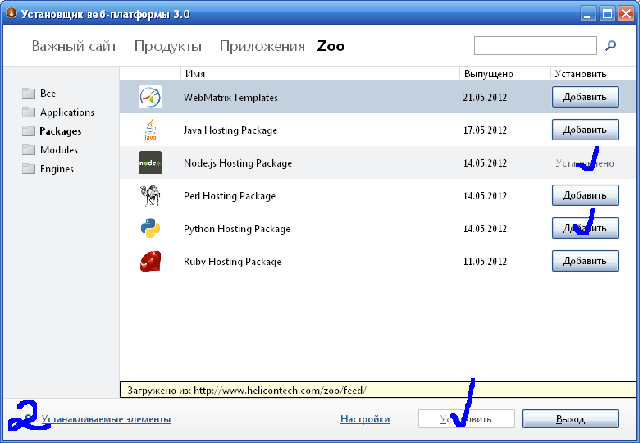
\includegraphics[width=11cm]{package_web}
	\end{center}
	\caption{Установка требуемых пакетов}
	\label{package_web}
\end{figure}
Далее устанавливаем WebMatrix Templates. На рис. ~\ref{fail_install} отображена возвращающаяся ошибка при установке.
\begin{figure}[!ht]
	\begin{center}
		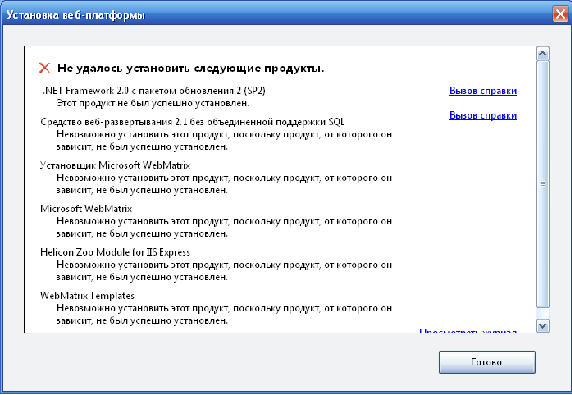
\includegraphics[width=11cm]{fail_install}
	\end{center}
	\caption{Возвращаемая ошибка}
	\label{fail_install}
\end{figure}
Никаких советов по исправлению этой проблемы найти не удалось. Установка таким способом пробовалась на Windows XP sp2 x64, sp3 x64 и x86. При удалении текущих версий .NET Framework никаких положительных изменений не происходило.  
Поэтому данный метод  также оказался неудачным.

\paragraph{Установка Node.js через Cygwin.}
Далее появилась идея избежать ошибки, выдаваемой командной строкой о выполнений sh, установкой node-ffi через Cygwin. 
Cygwin — UNIX-подобная среда и интерфейс командной строки для Microsoft Windows. Cygwin обеспечивает тесную интеграцию Windows приложений, данных и ресурсов с приложениями, данными и ресурсами UNIX-подобной среды. Из среды Cygwin можно запускать Windows приложения, также можно использовать инструменты Cygwin из Windows.

Cygwin состоит из двух частей: динамически подключаемая библиотека cygwin1.dll, которая обеспечивает совместимость API и реализует значительную часть стандарта POSIX и огромная коллекция приложений, которые обеспечивают привычную среду UNIX.

Стандарт Posix – это один из общепринятых стандартов повышения мобильности программного обеспечения (ПО).  Задача обеспечения мобильности ПО является очень важной задачей исключительной сложности. Едва ли стоит обосновывать это каким-либо более широким способом.
При установке Cygwin в каталог собирается Linux-подобный корневой каталог, представленный на рис. ~\ref{cygwin_catalogue}.
\begin{figure}[!ht]
	\begin{center}
		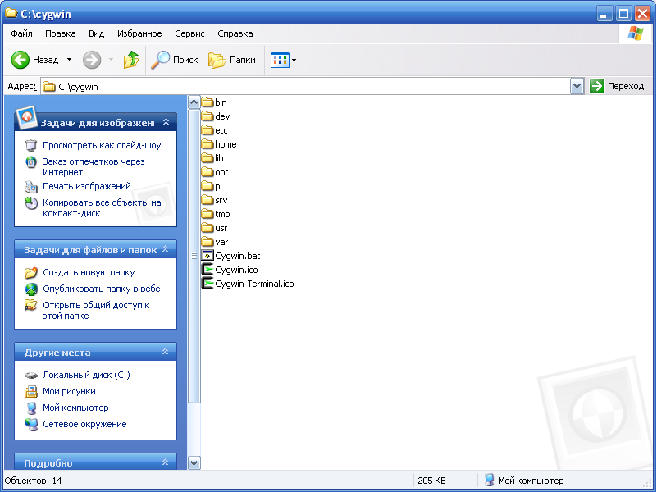
\includegraphics[width=11cm]{cygwin_catalogue}
	\end{center}
	\caption{Корневая папка Cygwin}
	\label{cygwin_catalogue}
\end{figure}

	При запуске Cygwin-Terminal открывается Terminal как в Linux, соответственно, если в его окружение установить всё, что надо (смотри пункт ~\ref{OnLinuxInstall}), то должен установиться node-ffi. Но возникла проблема с тем, что установка libffi тянет за собой, грубо говоря, весь Linux. Очень много времени было потрачено на попытки установки node-ffi через Cygwin, но результат не был достигнут.
\paragraph{Подведение итогов.} На данный момент решение данной проблемы придумано не было. Создателем платформы был отправлен запрос на помощь в установке node-ffi с подробным описанием проблем в установке.\\
Буквально на днях был получен ответ, в котором было сказано попробовать установить всё через Mozilla-Build, при этом скомпилировав в ней libffi. В условиях сдачи диплома на данный момент времени попробовать такой вариант нет. Работа над установкой node-ffi под Windows будет продолжена позднее.  Вообще говоря, большое количество программистов, использующих node.js сетуют на Node Package Manager, потому что он требует серьёзных предустановок и даже при этом не работает стабильно. \\
Существует предложение создать уже скомпилированные файлы для установки под каждую версию операционных систем, для того, чтобы не нужно было устанавливать такой большой объем программ. Кстати, в рамках нашего проекта, это может послужить большой проблемой, размещая сервер локально на каждом компьютере, будет необходимо установить большой объём информации. С одной стороны технология использования Node.js пока что не оправдала себя полностью , но ещё есть более полугода, возможно, разработчики исправят эту проблему, либо придётся компилировать всё своими руками. С другой стороны, размещение сервера удалённо решит эту проблему  и тут node.js, как уже было описано, подходит как нельзя кстати.\\
Нет волнений, что текущая идея может быть невыполнима, используя выбранные технологии.

\chapter{Реализация программы}
\section{Предварительная работа с динамической библиотекой}\label{base.txt}
Для того, чтобы при изменении динамической библиотеки не нужно было менять код программы было сделано следующее. В корневом каталоге с файлами, необходимыми для создания сервера, создаётся текстовый файл base.txt. Содержание файла формируется из информации о функциях, заявленных в динамической библиотеке. Каждая функция записывается в текстовый файл  следующим образом:
\begin{lstlisting}[numbers=none, language=bash]
"function name","return type","var's type",["var's type", [...]],
\end{lstlisting}
Сначала записывается имя функции, потом тип возвращаемого значения, далее перечисляются типы передаваемых переменных в фукнцию в том порядке, в котором они идёт в ней. В конце записи ставится запятая.
Следующая функция записывается со следующей строки.
После того как все функции описаны, на следующей строке записывается имя динамической библиотеки без расширения. После имени никаких символов не ставится. К созданной динамической библиотеке (см. пункт ~\ref{CreationDynLib}) файл base.txt будет выглядеть следующим образом:
 \lstinputlisting[frame=shadowbox, 
   emph={forsuffixes,text,bpath},emphstyle={\color{red}},
   emph={[2]fill,unfill},emphstyle={[2]\bfseries\underbar}
 ]{../base.txt}
В пункте ~\ref{projectStructure} описано, как используется этот файл.
\section{Оформление запроса}
Flash-приложение посылает запрос на сервер. Сервер разбирает этот запрос, выполняет нужную функцию из динамической библиотеке, и посылает результат выполнения ответов. Разберем, как организовать запрос на примере:
\begin{lstlisting}[numbers=none, language=bash]
"http://127.0.0.1:8888/>?int=subtraction+float=123.3+int=1"
\end{lstlisting}
\begin{itemize}
   \item http://127.0.0.1:8888/ - сайт, куда посылается запрос с портом, который прослушивает сервер;
   \item >? - данный символ указывает серверу на то, что этот запрос - это запрос на выполнение функции из подгружаемой динамической библиотеки;
  \item int=subtraction - тип возвращаемого значения и имя функции;
  \item float=123.3 - тип передаваемого параметра и его значения;
\end{itemize}
Между параметрами и описанием функции ставится \textbf{+}. Все передаваемые параметры должны быть перечислены строго в том порядке, в котором они заданы в функции из динамической библиотеки. Тип параметров должны в точности совпадать с типами передаваемых переменных, объявленных в функции.
На данном этапе разработки при неправильно созданном запросе, сервер пытается найти функцию с такими параметрами и, не находя её, аварийно завершает работу.
Существует следующие варианты того, как будет вести себя сервер при неверном запросе:
\begin{itemize}
  \item Пропускать данный запрос, не уведомляя об ошибке запроса.
  \item Возвращать ошибку.
\end{itemize}
Для программиста, который пишет Flash-программу, если он неверно задаёт запрос, для отладки важно, чтобы ему возвращалась ошибка, с указанием о том, какой запрос был создан неправильно. Поэтому выбран второй вариант. При этом важно сделать так, чтобы Flash-программисту было легко понять какой из запросов выдал ошибку, а также охрактеризовать тип ошибки, предложив пути решения. Данная проблема будет решена в следующих версиях моего проекта.
\section{Структура проекта}\label{projectStructure}
Весь проект делится на 2 части:
\begin{itemize}
  \item  Написать сервер, работающий с динамической библиотекой.
  \item Написать функцию в Flash для работы с запросом
\end{itemize}
\subsection{Серверная часть}\label{ServerPart}
Для серверной части написано три скрипта:
\begin{itemize}
  \item  http.js - Создание сервера;
  \item  readRequest.js - Разбор полученного запроса;
  \item text.js - Инициализация динамической библиотеки.
\end{itemize}
В text.js написана функция, которая на основе файла base.txt (см пункт ~\ref{base.txt}) подключает динамическую библиотеку. В readRequest.js написаны две функции. Функция GetReturnType(text) - возвращает тип возвращаемого значения функции. Функция Search(text, way) - возвращает массив, при этом если в параметр way указать значение "type", то массив будет состоять из типов передаваемых параметров. Если же передать "value" - массив значений, которые нужно передать в качестве параметров функции.
Рассмотрим работу библиотеки node-ffi на примере нашего проекта (см. ~\ref{text.js}).
 \lstinputlisting[frame=shadowbox,
   emph={forsuffixes,text,bpath},emphstyle={\color{red}},
   emph={[2]fill,unfill},emphstyle={[2]\bfseries\underbar}, caption=Код text.js. Инициализация динамической библиотеки, label={text.js}
 ]{../text.js}

Следующие строки подключают библиотеки для работы с динамическими библиотеками и для работы с файлами соответственно:
 \lstinputlisting[firstline =1, lastline=2,
   emph={forsuffixes,text,bpath},emphstyle={\color{red}},
   emph={[2]fill,unfill},emphstyle={[2]\bfseries\underbar}, 
 ]{../text.js}
В данном скрипте функция DynLib() формирует объект StructForLib для выгрузки из динамической библиотеки функций. Рис. ~\ref{StructForLib}показывает, как выглядит StructForLib перед выгрузкой из тестовой динамической библиотеки:
\begin{figure}[!ht]
	\begin{center}
		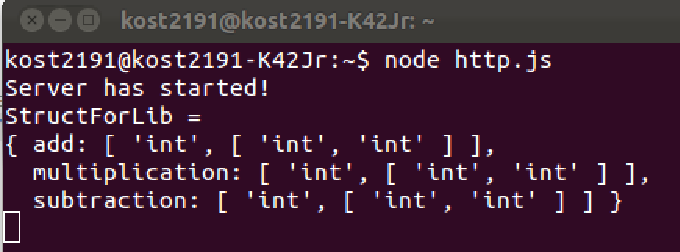
\includegraphics[width=11cm]{StructForLib}
	\end{center}
	\caption{Параметр для передачи в Library из node-ffi}
	\label{StructForLib}
\end{figure}
После того, как StructForLib был сформирован, по нему создается объект lib1 с методами, являющимися функциями динамической библиотеки:
 \lstinputlisting[firstline =40, lastline=40,
   emph={forsuffixes,text,bpath},emphstyle={\color{red}},
   emph={[2]fill,unfill},emphstyle={[2]\bfseries\underbar}, 
 ]{../text.js}
После этого в объекте lib1 станут достпуны методы: add(int, int), multiplication(int, int), subtraction(int, int).
Каждый раз при обработке запроса из lib1 будет вызываться метод, который был запрошен Flash-приложением.
 \lstinputlisting[frame=shadowbox,
   emph={forsuffixes,text,bpath},emphstyle={\color{red}},
   emph={[2]fill,unfill},emphstyle={[2]\bfseries\underbar}, caption=Код http.js. Сервер, label={http.js}
 ]{../http.js}
Сначала подключаются скрипты text.js, readRequest.js. Далее вызывается функция инициализации из text.js. После этого создается сервер, слушающий порт 8888. В котором каждый запрос с ">" обрабатывается и вызывается соответствующая функция, после чего сервер отправляет ответ, возвращаемый данной функцией.

\subsection{Клиентская часть РРРРРРРРРРРРРРРРРРРРРРРР}
Клиентом у нас в данном случае является приложение, написанно на ActionScript. При настройках Flash по умолчанию, он не может отправлять и получать данный с локальных серверов. Так как наш сервер поднимается локально, значит нужно поменять настройки flash. Рассмотрим типы изолированной программной среды безопасности, в которой работает вызывающий файл.
\begin{itemize}
  \item REMOTE: этот файл загружается с URL-адреса в Интернете и используется в соответствии с правилами изолированной программной среды на основе домена;
  \item LOCAL\_WITH\_FILE: этот файл является локальным файлом, не является доверенным для пользователя и не публиковался с сетевым наименованием. Файл может считывать информацию из локальных источников данных, но не может обмениваться данными через Интернет;
  \item LOCAL\_WITH\_NETWORK: этот SWF-файл является локальным файлом, не является доверенным для пользователя и публиковался с сетевым наименованием. SWF-файл может обмениваться данными через Интернет, но не может считывать информацию из локальных источников данных;
  \item LOCAL\_TRUSTED: этот SWF-файл является локальным файлом, пользователь сделал его доверенным с помощью диспетчера настроек проигрывателя Flash Player или файла конфигурации FlashPlayerTrust. Файл может считывать информацию из локальных источников данных и обмениваться данными через Интернет;
  \item APPLICATION: файл работает в приложении AIR и был установлен с пакетом (файлом AIR) для этого приложения. По умолчанию файлы в изолированной программной среде безопасности приложения AIR могут выполнять перекрестные сценарии с любым файлом из любого домена (в то время как файлы за ее пределами могут не иметь разрешения на выполнение перекрестных сценариев с файлом AIR). По умолчанию файлы в изолированной программной среде безопасности приложения AIR могут загружать содержимое и данные из любого домена. 
\end{itemize}

В случае работы программиста используется FlashPlayerDebugger из Flex SDK. Он позволяет эффективно отлаживать программу, в её теле ставить breakpoint'ы а также использовать функцию trace(), выводящую в консоль IntelliJ IDEA тот параметр, который мы передали в trace().
Для смены настроек изолированной среды, нужно перейти в папку с используемым Flash Player'ом и вызвать настройки.

НЕ НАЙТИ КАК ВЫЗВАТЬ НАСТРОЙКИ




\chapter{Установка сервера участником}
На данном этапе дипломной работы создан Shell Script для установки Node.js в Ubuntu.
В листинге ~\ref{nodejs.sh} представлен Shell Script для установки Node.js и компонентов, необходимых для правильной работы сервера. После скачивания всего проекта Конкурса вызывается это скрипт.
 \lstinputlisting[frame=shadowbox, caption=Команды для установки node.js через Терминал,
   label=nodejs.sh,
   emph={forsuffixes,text,bpath},emphstyle={\color{red}},
   emph={[2]fill,unfill},emphstyle={[2]\bfseries\underbar}
 ]{../installNodejsUbuntu/nodejs.sh}

Файлы, относящиеся к серверу, а также динамическая библиотека устанавливаются в домашнюю папку каталога.

\chapter{Заключение}
\section{Достигнутые результаты}
В процессе работы над дипломным проектом:
\begin{itemize}
  \item Изучено программное обеспечение конкурса КИО.
  \item Проанализированы достоинства и недостатки различных платформ, которые можно было использовать для реализации сервера. В итоге выбран Node.js и обосновано его использование;
  \item Спроектирована общая структура сервера, выбраны протоколы обмена между частями системы;
  \item Для вызова функций из динамической библиотеки используется модуль node-ffi;
  \item Описана процедура установки и настройки node-ffi под Linux;
  \item Под Windows установить этот модуль не удалось. Попытки описаны в ВЫАПТЛЫВАТПШ. 
  \item Реализован сервер на Javascript, который принимает запросы, вызывает нужные функции и возвращает результат;
  \item Реализован пример на Flash, который демонстрирует соединение приложения с динамической библиотекой через созданный сервер.
  \item Код протестирован и отвечает поставленном в техническом задании требованиям. Код прокомментирован и документирован в этой пояснительной записке.
  \item Создан Shell Script для установки node.js для Ubuntu. При сборке всего установщика конкурса при выполнении данного скрипта будет установлен вся серверная часть. 
\end{itemize}
\section{Дальнейшее развитие проекта}
\begin{itemize}
  \item Реализация сервера под Windows (создание скомпилированных версий node-ffi под каждую версию Windows);
  \item Обработка ошибок при создании запроса программистом, создающим Flash-приложение для удобства отладки программистом.
  \item Создание утилиты, которая извлекает сведения о функциях из динамической библиотеке и приводит данные к формату base.txt.
\end{itemize}

\chapter{Используемая литература}
При создании дипломной работы была использована следующая литература, сайты, видео:

\begin{enumerate}
  \item  Книжку про Adobe Flex добавить кто и что
  \item  Документация Node.js: http://nodejs.org/api/
  \item Подробный учебник по Node.js: http://nodebeginner.ru/;
  \item Видео Ryan'а Dahl'a: Знакомство с Node.js: \\
http://www.youtube.com/watch?v=jo\_B4LTHi3I;
  \item Политика безопасности в Flash Player:\\ http://kharchuk.ru/as3/Security.html;
  \item Cоздание динамической библиотеки в Linux:\\ http://www.firststeps.ru/linux/general1.html;
  \item Документации пакетов LaTeX disser, listings:\\ http://ru.wikipedia.org/wiki/LaTeX а также примеры внутри пакетов.
  \item Книга по Javascript
  \item Методичка по оформлению диплома
\end{enumerate}

\bibliography{thesis}
\bibliographystyle{gost705}
\end{document}

